\chapter{Encapsulator}\label{encapsulator}

This module is designed to create the encapsulated modules as described the specification.
The standard encapsulation structure is the following:
\begin{table}[H]
    \centering 
    \begin{tabularx}{\textwidth}{|c|c|>{\centering\arraybackslash}X|} 
        \hline
        Field name  & Bits      & Description \\ \hline
        header      & 8         & Encapsulation header. \\ \hline
        srcID       & 0 - 16    & Source ID. \\ \hline
        timestamp   & T*8       & Time stamp.\\ \hline
        payload     & 1 - 248   & Packet payload \\ \hline    
    \end{tabularx}
    \caption{Encapsulation field groups} 
    \label{tab:encapsulation_groups}
\end{table}

As clearly explicited in the specification: the uppermost field must be transmitted first and 
multi-bit fields are transmitted least significant bit first.

This module is a simple combinatorial network that takes the inputs from the TE and configuration 
registers and puts them inside the associated structs (when necessary).

\section{Header}
The header is a byte long and works as an introduction to the payload.
It is organized as follows:
\begin{table}[H]
    \centering 
    \begin{tabularx}{\textwidth}{|c|c|>{\centering\arraybackslash}X|} 
        \hline
        Field name  & Bits  & Description \\ \hline
        length      & 5     & Encapsulated payload length. A value of L indicates an L byte 
                              payload. Must be > 0.  \\ \hline
        flow        & 2     & Flow indicator. This can be used to direct packets to a particular 
                              sink in systems where multiple sinks exist, and those sinks include 
                              the ability to accept or discard packets based on the flow value. \\ \hline
        extend      & 1     & Indicates the presence of timestamp when 1. Must be 0 if timestamp 
                              width is 0. \\ \hline
    \end{tabularx}
    \caption{Header fields} 
    \label{tab:header}
\end{table}

The header is implemented as a \texttt{packed struct} in system verilog, this way each field can be 
accessed via dot notation.

\section{srcID}
This fields serves as an identification for the packet source and its size varies from 0 to 16 
bits.
As explained in the specification, this field can be omitted for two particular scenarios:
\begin{itemize}
    \item   There's only one source in the system.
    \item   The transport scheme uses a sideband bus for the source ID (for example, ATB). 
\end{itemize}

Since in this implementation we have only one source - the TE - and the transport used is ATB, 
there's no need for this field.

\section{Timestamp}
THis field is used to include time information with every packet. It is included in the 
encapsulation if header.extend is 1. When included it is T bytes long.
The timestamp field can be omitted if the user is not interested or it is already included inside 
the payload. To verify if the timestamp is included within the payload it looks into the TE 
configuration parameters.

\section{Payload}
The encapsulation payload has the following structure:
\begin{table}[H]
    \centering 
    \begin{tabularx}{\textwidth}{|c|c|>{\centering\arraybackslash}X|} 
        \hline
        Field name      & Bits      & Description \\ \hline
        type            & $\geq 0$  & Packet type. May be eliminated for sources with only on 
                                      packet type. \\ \hline
        trace\_payload  & $\leq R$  & Packet payloads such as those defined for E-Trace. Maximum 
                                      value of R is defined as 248 - Y - srcID\%8 where Y is the 
                                      length of the type field. \\ \hline
    \end{tabularx}
    \caption{Payload fields} 
    \label{tab:payload}
\end{table}

As explained in the specification, if the TE implemented supports only the \textit{instruction 
tracing} (like in our case), the \textit{type} field can be omitted from payload.
The length of the \textit{trace\_payload} field in this implementation is the maximum allowed 
(248) beacause both the type and srcID fields are omitted.

\section{Null Encapsulation}
The specification also describes the \textit{null packets}, they can be distinguished by standard 
packets from the length field field of the header that is set to 0. 
This family of packets is used for those transport schemes that do not use a ready/valid 
handshake, but instead they a require a continuous flow of data and when there is no useful data 
the gaps are filled by null packets.

In this implementation it was chosen to use the ATB transport protocol, that uses a ready/valid 
handshake and so the null packets are not emitted at all.

For completeness, it is the reported the two kinds of null packets:
\begin{itemize}
    \item   \textit{null.idle}, used to fill gaps.
    \item   \textit{null.alignment}, used for synchronization.
\end{itemize}

To discriminate between the two types it is used the extend field of the header, that otherwise 
it would have been useless.

\begin{figure}[H]
    \centering
    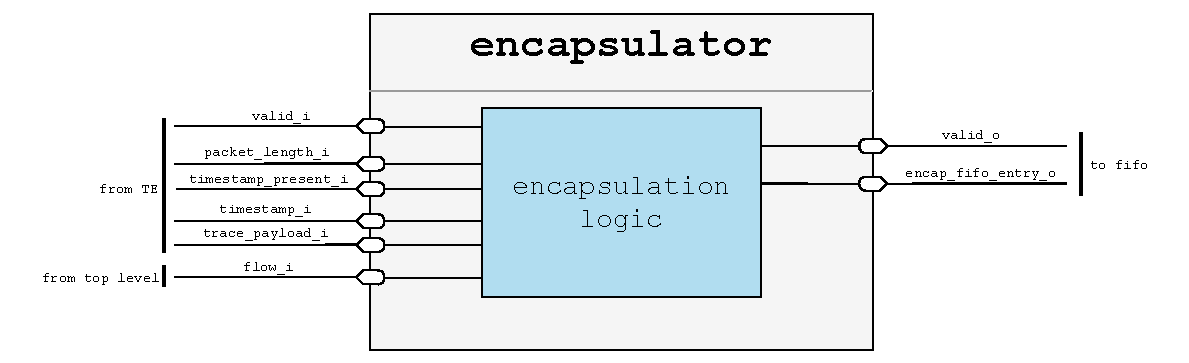
\includegraphics[width=1\textwidth]{img/encapsulator.pdf}
    \caption{Encapsulator internal architecture}
    \label{fig:encapsulator_internal_architecture}
\end{figure}